% ****** Start of file apssamp.tex ******
%
%   This file is part of the APS files in the REVTeX 4.2 distribution.
%   Version 4.2a of REVTeX, December 2014
%
%   Copyright (c) 2014 The American Physical Society.
%
%   See the REVTeX 4 README file for restrictions and more information.
%
% TeX'ing this file requires that you have AMS-LaTeX 2.0 installed
% as well as the rest of the prerequisites for REVTeX 4.2
%
% See the REVTeX 4 README file
% It also requires running BibTeX. The commands are as follows:
%
%  1)  latex apssamp.tex
%  2)  bibtex apssamp
%  3)  latex apssamp.tex
%  4)  latex apssamp.tex
%
\documentclass[%
reprint,
%superscriptaddress,
%groupedaddress,
%unsortedaddress,
%runinaddress,
%frontmatterverbose, 
%preprint,
%preprintnumbers,
%nofootinbib,
%nobibnotes,
%bibnotes,
amsmath,amssymb,
aps,
%pra,
%prb,
%rmp,
%prstab,
%prstper,
%floatfix,
]{revtex4-2}

\usepackage{graphicx}% Include figure files
\usepackage{dcolumn}% Align table columns on decimal point
\usepackage{bm}% bold math
\usepackage{zref-user} % don't even know what I use this for
\usepackage{hyperref}
\usepackage{placeins}

%\usepackage[mathlines]{lineno}% Enable numbering of text and display math
%\linenumbers\relax % Commence numbering lines

%\usepackage[showframe,%Uncomment any one of the following lines to test 
%%scale=0.7, marginratio={1:1, 2:3}, ignoreall,% default settings
%%text={7in,10in},centering,
%%margin=1.5in,
%%total={6.5in,8.75in}, top=1.2in, left=0.9in, includefoot,
%%height=10in,a5paper,hmargin={3cm,0.8in},
%]{geometry}

\begin{document}
	
	\preprint{APS/123-QED}
	
	\title{Determining the Specific Heat of Gadolinium}
	
	
	\author{Duncan Cayenne-McCall}
	\affiliation{Case Western Reserve University}
	
	
	\date{\today}% It is always \today, today,
	%  but any date may be explicitly specified

	
	\begin{abstract}
		 Abstract goes here.
		
	\end{abstract}
	\maketitle
	\section{\label{sec:level1}Introduction}
	The heat capacity of gadolinium (Gd), the 64\textsuperscript{th} element is of interest due to its ferromagnetic properties. Gadolinium is known to have a spontaneous magnetic moment below its Curie temperature $T_C$, which means that there exist macroscopic regions in which the atomic magnetic moments are aligned. As we will soon see, this spontaneous magnetic moment has interesting thermodynamic implications. 
	
	\subsection{\label{sec:level2}Ising Model Thermodynamics}
	In the Ising thermodynamic model, a given material can be modeled as a grid or lattice with each vertex representing the location of an atom with spin $\pm1/2$. Each vertex thus has a potential energy if it is antiparallel with its neighboring spins\cite{UT}, and negative when it is parallel. Assuming our material is not in the presence of an external magnetic field, if it goes from having no net magnetization to ferromagnetic, we would expect to observe a spontaneous drop in system energy. It is this instantaneous drop in energy that results in a sharp kink in the curve of energy versus temperature.
	
	The heat capacity of a system describes its ability to increase in energy without also experiencing a large change in temperature. This value is also often reported to be per unit mass. From this we conclude that excluding any external sources or drains of energy, the heat capacity can be represented as the derivative of a energy temperature plot. The kink at $T_C$ in the aforementioned plot of energy vs. temperature results in a discontinuity of the heat capacity versus temperature. Given that we gain a discontinuity in the derivative of our order parameter, the behavior at and around $T_C$ represents a second order transition\cite{UT}.
	
	\section{\label{sec:level1}Apparatus and Procedure}
	
	
	\subsection{\label{sec:level2}Gadolinium Apparatus}
	Our gadolinium sample was a cylinder $11\pm2mm$ tall with a $7\pm2mm$ radius, and was placed within a vacuum chamber. Attached to the gadolinium sample and also within the vacuum chamber was a heating coil, which we could use to increase the sample energy. In contact with the gadolinium was a brass post smaller than the sample, and the post itself was attached to a large aluminum cylinder  which was outside of the vacuum region. 
	
	To measure the temperature of our sample, we used Vishay thermistors and a spline to interpolate the manufacturer's temperature vs. resistance data points. To measure the heat capacitance at various temperatures, we first had to bring the sample to a steady temperature, which we did by bringing it and the aluminum stage into equilibrium. The aluminum stage could be cooled or heated using a thermoelectric cooler attached to its base. Its cooling performance could be further improved by cryogenically cooling its base.
	
	We utilized two Keithley digital multimeters via a single serial GPIB line to take time series measurements that allowed us to better understand the temporal behavior of the system. The Keithley 2000 multimeters were limited in their measurement frequency, allowing us to collect resistance measurements for both the sample and the stage every $\approx1.5s$. However, this was not a limiting factor in our experiment as any meaningful changes in temperature happened over the course of minutes. 
	
	
	\begin{figure}
		\centering
		\includegraphics[width=1\linewidth]{../../../Downloads/gadolinium2ApparatusCropped}
		\caption{The apparatus of our g
			gadolinium sample and associated equipment.}
		\label{fig:gadolinium2apparatuscropped}
	\end{figure}
	
	
	\subsection{\label{sec:level2}Thermoelectric Cooler ``P''ID Controller}
	Our heat capacity measurements involved bringing the sample to a steady temperature, heating it with the coil, and calculating the amount of energy that went from the coil to the sample. Given that both the sample and coil are in vacuum, the energy that goes into the sample is simply the heater power multiplied by the on time. However, the gadolinium dissipates some of its heat through the brass rod to the aluminum stage. We mitigate this by starting them at the same temperature.
	
	Keeping the aluminum stage at a fixed temperature required writing a control loop. Given that we could not switch the polarity of the thermoelectric cooler, we had to choose between active cooling or heating for a given trials. For target temperatures above room temperature we used active heating and simply allowed it passively cool if we overshot the target. The same method worked vice-versa for target temperatures below room temperature. The downside of this is that we get asymmetric performance when balancing about our target temperature, resulting in oscillations that are challenging to dampen.
	
	As mentioned previously, meaningful changes in temperature occurred on the order of minutes, which has both benefits and drawbacks. The system had plenty of time to react to errors, but also responded slowly. The slow response additionally made it challenging to evaluate the performance of a given controller parameter. We began with a proportional controller tuned to the best of our abilities, and added a quadratic term to reduce the response at small errors. Ultimately, many oscillations remained, though they were often centered near the target temperature with amplitudes no greater than $0.2^{\circ} C$.
	
	\subsection{\label{sec:level2}System Thermodynamics}
	For any given measurement, the gadolinium sample, brass post, and aluminum stage are all in equilibrium with one another. However, once the heater coil turns on, the gadolinium sample heats up, and a temperature differential forms across the brass post. The brass post then dissipates heat from the sample to the aluminum stage, which is so massive as to be considered a thermal bath, and is at a constant temperature. The rate of energy dissipation follows Newton's law of cooling
	\begin{equation}
	\frac{Q}{t} = \frac{kA\Delta T}{d}
	\end{equation}	
	which says that the heat per unit time is equivalent to the thermal conductivity $k$ times the cross-sectional area $A$ times the temperature gradient $\Delta T/d$, where d is the distance across the sample. The instant the heater turns on, the brass post dissipates energy from the gadolinium at a slow rate. As the heater stays on for a large time $t$, the temperature gradient across the post reaches a value such that the rate of dissipation is the same as the energy being added through the heater coil, and the gadolinium reaches a steady temperature.
	
	When the gadolinium has a small heat capacity, for the same power, we expect it will rise more quickly in temperature and reach the steady state more quickly, and vice versa for a small heat capacity. 
	
	We can model the behavior of temperature as a function of time using a differential equation.
	\begin{equation}
		\frac{dT}{ds}=\frac{1}{H}\left(P_{in}-\frac{kA}{d}\frac{(T(s)-T_{Base})}{1}\right)
	\end{equation}
	This equation says that the rate of temperature $(T)$ change at a time $(s)$ is equivalent to the power at a given time divided by the heat capacity $H$. $T_{Base}$ is used to define the temperature differential, and is taken to be a constant, as the energy dissipated to the aluminum block raises its temperature negligibly.
	
	The solution to this differential equation takes the following form, though the y shift constants were combined when doing curve fitting. Additionally, while the values of A and d are theoretically known, these values were folded into a constant due to their uncertainty.
	
	\begin{equation}
		T(s) = T_{Base} + \frac{P_{in}}{A} - Cexp\left(\frac{As}{H}\right)
	\end{equation}
	
	Most importantly the inverse heat capacity shows up in the exponent, which means a small heat capacity will rise quickly and a large heat capacity will rise slowly. We can additionally determine the heat capacity by performing a linear fit on the region immediately after the heater turns on, when the dissipation rate is low. We can solve for the heat capacity 
	\begin{equation}
		\frac{1}{slope}\times Power = \frac{seconds}{degree}\frac{Joules}{second} = \frac{Joules}{degree}.
	\end{equation}
	
	
	\section{\label{sec:level1}Results and Analysis}
	We performed our measurements in single degree increments about 21\textdegree C, which was where a supposed phase transition occurs in gadolinium\cite{Bednarz}. We will first discuss the results of the linear approximation method.
	\subsection{\label{sec:level2}Linear Approximation Method}
	One liberty taken in this method is that the reported measurements are shown to be in units of $J/K$, and not reported to be a heat capacity per unit mass, which can be justified. Due to our inability to get proper measuring devices on the gadolinium sample itself, the uncertainty in its dimensions were large compared to the size of the sample. These errors are further exacerbated by the fact that volume error scales cubically with the measured dimension, resulting in a large mass uncertainty. Furthermore, reporting a per-mass unit heat capacity implies all samples behave the same regardless of dimension, which they do not. On top of this, we have sought out relative changes in heat capacity near the Curie temperature and less so an absolute value.
	
	\begin{figure}
		\centering
		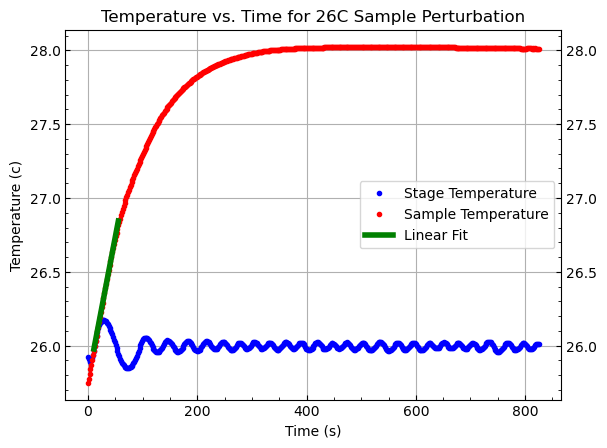
\includegraphics[width=1\linewidth]{26Cperturbation2}
		\caption{Time dependence of temperature when sample and stage begin at 26C. Also contains the linear approximation for times near the start time.}
		\label{fig:26cperturbation2}
	\end{figure}
	
	In figure (2) we see an example of what a test for a given temperature looked like. Note the small oscillations of the aluminum stage temperature centered about the target of 26\textdegree C. We chose to perform a linear fit on the region close to $t=0$. The x axis times also provide perspective on the slow nature of the experiment, taking nearly five minutes to reach its equilibrium temperature, which was very near 2\textdegree C above the target temperature. 
	
	\begin{figure}
		\centering
		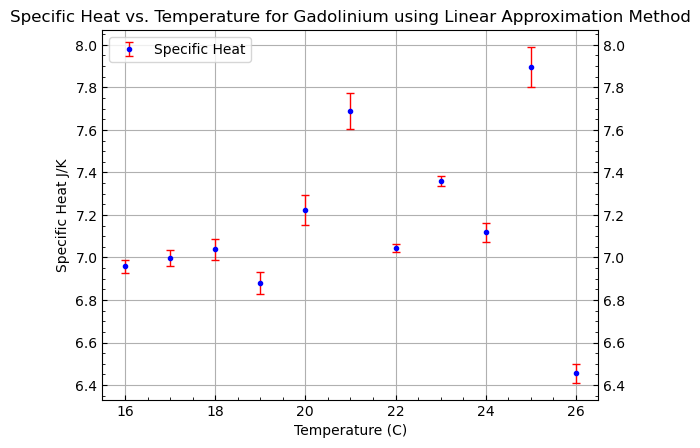
\includegraphics[width=1\linewidth]{download}
		\caption{The specific heat of Gadolinium versus the temperature of the sample observed on a range of 16C to 26C.}
		\label{fig:download}
	\end{figure}
	
	Shown in figure (3) is the result of the specific heat versus temperature observed using the linear approximation method. While we observe a somewhat decaying pattern centered about 21\textdegree C, we can hardly conclude that this is our Curie temperature due to the large fluctuating behavior at 19\textdegree C and 23\textdegree C respectively. From this data alone, it is challenging to conclusively state that the ferromagnetic transition of gadolinium is of first or second order. We observed the maximum specific heat of our sample to be 
	
	
	
	
	

	
	
	
	
	\begin{acknowledgments}
	I would like to thank my lab partner Benjamin Mellick and professors Dr. Monreal and Dr. Martens for their guidance in completing this experiment.  
	\end{acknowledgments}
	
	
	\begin{thebibliography}{13} % Assuming no more than 9 
	\bibitem{UT} Richard Fitzpatrick, The Ising Model, University of Texas at Austin, 2006
	\bibitem{Bednarz} Grzegorz Bednarz, Heat Capacity of Gadolinium near the Curie temperature, Physical Review B,  1993.
	\bibitem{Lanchester} P. C. Lancheste, The Critical Specific Heat of Gadolinium, Journal of Magnetism and Magnetic Materials, 1980.
	\end{thebibliography}
	
	
	

\end{document}
%
% ****** End of file apssamp.tex ******
